% =============================================================================
% Replacement for §5.2 (the GaGa Model for Differential Expression) of the
% PIG paper. Drop in as a single subsection. References to \cite{} should
% be present in the surrounding paper's bib (Rossell2009GaGa, Kendziorski2003Parametric,
% Armstrong2002, MAQC2006, Smyth2004limma). Two figure files are referenced:
%   figs/alpha_sweep_pp_diff.pdf
%   figs/scatter_pp_vs_gold.pdf
% Place those next to the .tex.
% =============================================================================

\subsection{The GaGa Model for Differential Expression}\label{sec:gaga}

\citet{Rossell2009GaGa} introduced the Gamma-Gamma (GaGa) hierarchical model
for differential expression analysis. For gene $i \in \{1,\dots,G\}$,
group $g \in \{1,\dots,K\}$, and replicate $j$, GaGa specifies
\begin{equation}\label{eq:gaga.model}
\begin{aligned}
x_{ijg} \mid \alpha_i, \lambda_{i,c_h(g)}
   &\sim \Ga\!\left(\alpha_i,\; \alpha_i / \lambda_{i,c_h(g)}\right),\\
1/\lambda_{ic} \mid a_0, \nu &\sim \Ga(a_0,\; a_0/\nu),\\
\alpha_i \mid b_\alpha, \nu_\alpha &\sim \Ga(b_\alpha,\; b_\alpha/\nu_\alpha),\\
z_i \mid \boldsymbol\pi &\sim \mathrm{Cat}(\boldsymbol\pi),
\end{aligned}
\end{equation}
where $z_i = h \in \{0,\dots,H-1\}$ is a latent pattern indicator that
partitions the $K$ groups into clusters $c \in \mathcal{C}_h$ (e.g., the
``equally expressed'' (EE) pattern groups all conditions together; the
``differentially expressed'' (DE) pattern places each group in its own
cluster). The shape parameter $\alpha_i$ is gene-specific and shared across
groups under the standard \texttt{equalcv=TRUE} setting. The differential
expression problem is to compute $\Pr(z_i \neq 0 \mid \mathbf{x}_i,
\boldsymbol\theta)$ for each gene, where $\boldsymbol\theta = (a_0, \nu,
b_\alpha, \nu_\alpha, \boldsymbol\pi)$ are common hyperparameters.

\subsubsection{The integrated marginal likelihood and its analytic obstacle}

Conditional on $z_i = h$ the latent rates $1/\lambda_{ic}$ can be integrated
out in closed form. Writing $n_{ic} = \#\{(j,g) : g \in c\}$,
$S_{ic} = \sum_{j, g \in c} x_{ijg}$,
$L_{ic} = \sum_{j, g \in c} \log x_{ijg}$, and $r_0 = a_0/\nu$, the
per-cluster marginal likelihood is
\begin{equation}\label{eq:m.cluster}
m_{ic}(\alpha) = \frac{\alpha^{n_{ic}\alpha}\,e^{(\alpha-1)L_{ic}}}{\Gamma(\alpha)^{n_{ic}}}
\cdot \frac{r_0^{a_0}}{\Gamma(a_0)}
\cdot \frac{\Gamma(a_0 + n_{ic}\alpha)}{(r_0 + \alpha S_{ic})^{a_0 + n_{ic}\alpha}}.
\end{equation}
The pattern-conditional marginal is $m_{ih}(\alpha) = \prod_{c \in
\mathcal{C}_h} m_{ic}(\alpha)$, and the gene-level pattern posterior is
\begin{equation}\label{eq:pp.gene}
\Pr(z_i = h \mid \mathbf{x}_i, \boldsymbol\theta) \;\propto\;
   \pi_h \int_0^\infty m_{ih}(\alpha)\, p(\alpha \mid b_\alpha, \nu_\alpha)\, d\alpha.
\end{equation}
The integrand involves $\Gamma(\alpha)^{-n_{ic}}$ and
$\Gamma(a_0+n_{ic}\alpha)$, so the integral has no closed form.
\citet{Rossell2009GaGa} addressed this by approximating $\log\Gamma(\alpha)$
with Stirling's formula and fitting the resulting integrand by a gamma
distribution; the moments of that gamma are then used inside an EM step
for $\boldsymbol\theta$. This Stirling approximation is reasonable for
large $\alpha$ but degrades for $\alpha$ close to zero, the very regime
of interest for high-CV expression data.

\subsubsection{P-IG-augmented exact MCMC for the gene-level posterior}

We replace the Stirling step with an exact MCMC scheme that targets
\eqref{eq:pp.gene} directly under the same hyperparameters
$\boldsymbol\theta$ produced by \texttt{gaga::fitGG}'s \texttt{quickEM}.
The ingredients are the P-IG identity for $\Gamma(\alpha)^{-N}$
\citep[Theorem~\ref{thm:main}]{} and the standard gamma identity for
$\Gamma(a_0 + n_c \alpha)$. Concretely, conditional on the augmenting
variables
\begin{equation}\label{eq:gaga.aug}
\begin{aligned}
\omega_s \mid \alpha_i &\stackrel{\mathrm{iid}}{\sim} \mathrm{P\text{-}IG}(\alpha_i),
   \quad s = 1, \dots, N_i = \!\!\sum_{c \in \mathcal{C}_h}\!\! n_{ic},\\
\tau_c \mid \alpha_i &\sim \Ga(a_0 + n_c \alpha_i,\; 1), \quad c \in \mathcal{C}_h,
\end{aligned}
\end{equation}
the conditional density of $\alpha_i$ factors as
\begin{equation}\label{eq:gaga.cond}
p(\alpha_i \mid \boldsymbol\omega, \boldsymbol\tau, z_i, \mathbf{x}_i, \boldsymbol\theta)
\;\propto\; \alpha_i^{\,N_i + b_\alpha - 1}\, e^{-\Omega \alpha_i^2 + B \alpha_i}
\cdot e^{R(\alpha_i)},
\end{equation}
with $\Omega = \sum_s \omega_s$,
$B = N_i\gamma + \sum_c L_c - b_\alpha/\nu_\alpha + \sum_c n_c \log \tau_c$,
$\gamma = -\psi(1)$, and a residual
$R(\alpha) = N_i \alpha \log \alpha - \sum_c (a_0 + n_c \alpha) \log(r_0 + \alpha S_c)$
that the augmentation cannot absorb. Because the augmentation handles
$\Gamma(\alpha)^{-N_i}$ and $\Gamma(a_0 + n_c \alpha)$ exactly, $R$ is the
\emph{only} place where the original Stirling difficulty would resurface.

To sample $\alpha_i$ from \eqref{eq:gaga.cond} we work on
$y_i = \log\alpha_i$ and use stepping-out plus shrinkage slice sampling
\citep{Neal2003slice} on
\begin{equation}\label{eq:gaga.ell}
\ell(y) = (N_i + b_\alpha)\,y - \Omega e^{2y} + B e^y + R(e^y),
\end{equation}
which is exact MCMC for the augmented target. The pattern indicator $z_i$
is updated with its closed-form full conditional
$\Pr(z_i = h \mid \alpha_i, \mathbf{x}_i, \boldsymbol\theta)
   \propto \pi_h\, m_{ih}(\alpha_i)$. After burn-in, posterior pattern
probabilities are estimated by Rao--Blackwellisation:
\begin{equation}\label{eq:rb.pp}
\widehat{\mathrm{pp}}_{ih} = \frac{1}{T - T_b}\,
   \sum_{t = T_b+1}^T \Pr\!\bigl(z_i = h \,\big|\, \alpha_i^{(t)}, \mathbf{x}_i, \boldsymbol\theta\bigr).
\end{equation}
The hyperparameters $\boldsymbol\theta$ are kept identical to those
produced by \texttt{gaga::fitGG}'s standard EM; only the posterior step
that gaga handles by Stirling is replaced.

\subsubsection{Simulation: when does the Stirling step matter?}

We compare \texttt{gaga::fitGG} (Stirling) and our P-IG-MCMC
implementation against a numerical-integration gold standard, all
evaluated at the same hyperparameters $\boldsymbol\theta$ obtained from
\texttt{quickEM}. Data are generated from \eqref{eq:gaga.model} via
\texttt{gaga::simGG}, which samples exactly from the assumed model.
Four scenarios cross the gamma-shape regime that controls Stirling
accuracy ($\nu_\alpha$, the prior mean of $\alpha_i$) with the per-group
sample size $n$ that controls $n_c \alpha_i$ inside the awkward
$\Gamma(a_0 + n_c \alpha)$ factor:

\smallskip
\begin{center}\footnotesize
\renewcommand{\arraystretch}{1.05}
\begin{tabular}{@{}lccccc@{}}
\toprule
Scenario & Description & $\nu_\alpha$ & $n$/group & $a_0$ & $\nu$ \\
\midrule
A (Easy)    & Microarray-like, low CV  & $20$ & $10$ & $20$ & $5$ \\
B (Medium)  & Bulk-RNA-seq-like        & $5$  & $5$  & $10$ & $5$ \\
C (Hard)    & High-overdispersion      & $1.5$& $4$  & $5$  & $5$ \\
D (Extreme) & Single-cell-like         & $0.5$& $3$  & $3$  & $5$ \\
\bottomrule
\end{tabular}
\end{center}
\smallskip

For each scenario we run $B = 10$ replicates with $G = 200$ genes, DE
prevalence $0.20$, and FDR threshold $0.05$. The gold standard pp is
computed by 600-point adaptive log-$\alpha$ quadrature applied to the
exact integrand of \eqref{eq:pp.gene}; the P-IG MCMC chain runs for
$T = 200$ iterations with $T_b = 60$ burn-in and PIG truncation
$N_{\mathrm{trunc}} = 30$.

Table~\ref{tab:gaga.sim.headline} summarises gaga's quickEM
hyperparameter recovery and the per-scenario discrepancy of each method
to the gold-standard posterior probabilities. The Stirling discrepancy
$\overline{|\Delta\mathrm{pp}|}_{\text{gaga}}$ grows by three orders of
magnitude from scenario~A to scenario~D ($4{\times}10^{-6} \to
2.7{\times}10^{-3}$); the P-IG MCMC discrepancy
$\overline{|\Delta\mathrm{pp}|}_{\text{PIG}}$ stays at the MCMC noise
floor of $\sim\!10^{-3}$ uniformly. In scenarios C and D, P-IG MCMC is
already several times closer to gold than gaga's Stirling.

\begin{table}[t]
\centering
\caption{Simulation: hyperparameter recovery (top) and per-scenario
posterior probability accuracy (bottom). Errors are mean absolute
deviation from the gold-standard posterior $\overline{|\Delta\mathrm{pp}|}$
together with Spearman correlation of the gene scores $1 - \mathrm{pp}_{i,0}$.
Each row is averaged over $B = 10$ independent replicates.}
\label{tab:gaga.sim.headline}
\smallskip
\renewcommand{\arraystretch}{1.05}
\setlength{\tabcolsep}{4pt}
{\footnotesize
\begin{tabular}{@{}lcccccccc@{}}
\toprule
\multicolumn{3}{c}{Oracle $\theta$} & \multicolumn{4}{c}{quickEM estimate} & & \\
\cmidrule(r){1-3}\cmidrule(lr){4-7}
Scen. & $\nu_\alpha$ & $a_0$ & $\hat{a}_0$ & $\hat{\nu}$ & $\hat{b}_\alpha$ & $\hat{\nu}_\alpha$ &  & \\
\midrule
A & 20  & 20 & 20.5 & 5.02 & 21.1 & 19.8 &  & \\
B & 5   & 10 & 10.5 & 5.04 & 8.74 & 5.16 &  & \\
C & 1.5 & 5  & 4.58 & 5.11 & 4.54 & 1.48 &  & \\
D & 0.5 & 3  & 2.56 & 5.50 & 9.00 & 0.44 &  & \\
\midrule
Scen. & \multicolumn{2}{c}{$\overline{|\Delta\mathrm{pp}|}$ vs.\ gold}
        & \multicolumn{2}{c}{Spearman vs.\ gold}
        & \multicolumn{2}{c}{empirical FDR}
        & \multicolumn{2}{c}{power} \\
\cmidrule(r){2-3}\cmidrule(lr){4-5}\cmidrule(lr){6-7}\cmidrule(lr){8-9}
& gaga & PIG-MCMC & gaga & PIG-MCMC & gaga & PIG-MCMC & gaga & PIG-MCMC \\
\midrule
A & $4.1\!\times\!10^{-6}$ & $9.1\!\times\!10^{-3}$ & $1.0000$ & $0.9960$
  & $0.056$ & $0.059$ & $0.417$ & $0.425$ \\
B & $2.1\!\times\!10^{-4}$ & $7.0\!\times\!10^{-3}$ & $1.0000$ & $0.9977$
  & $0.082$ & $0.079$ & $0.065$ & $0.072$ \\
C & $1.7\!\times\!10^{-3}$ & $3.4\!\times\!10^{-3}$ & $0.9970$ & $0.9990$
  & $0.000$ & $0.000$ & $0.005$ & $0.005$ \\
D & $2.7\!\times\!10^{-3}$ & $5.4\!\times\!10^{-4}$ & $0.9652$ & $0.9996$
  & $0.000$ & $0.000$ & $0.000$ & $0.000$ \\
\bottomrule
\end{tabular}}
\end{table}

The downstream consequence on differential-expression detection at
$\mathrm{FDR} = 0.05$ is small in scenarios with sufficient signal
(A, B): both methods give nearly identical empirical FDR and power.
In scenarios C and D the data carry too little information for either
method to flag genes at $0.05$, but the AUC of the gene scores tracks
how well the rankings match the truth: gaga has $0.594$ in scenario D
versus $0.600$ for both gold and P-IG MCMC, a small but systematic
gap caused by Stirling skewing the small-$\alpha$ tail.

To map the boundary cleanly we sweep $\nu_\alpha$ at fixed
$n = 5$ and otherwise constant hyperparameters
(Figure~\ref{fig:gaga.sweep}). The Stirling error
$\overline{|\Delta\mathrm{pp}|}_{\text{gaga}}$ grows from below
$10^{-5}$ at $\nu_\alpha \ge 8$ to over $5\!\times\!10^{-3}$ at
$\nu_\alpha = 0.5$, while the P-IG MCMC error stays bounded by its
$O(1/\sqrt{T})$ MCMC noise of $\sim\!7\!\times\!10^{-3}$ across the
entire grid. The two curves cross near $\nu_\alpha \approx 2$: above
this, Stirling is essentially exact and slightly more efficient than
finite-iteration MCMC; below, exact MCMC is meaningfully closer to
the truth.

\begin{figure}[t]
\centering
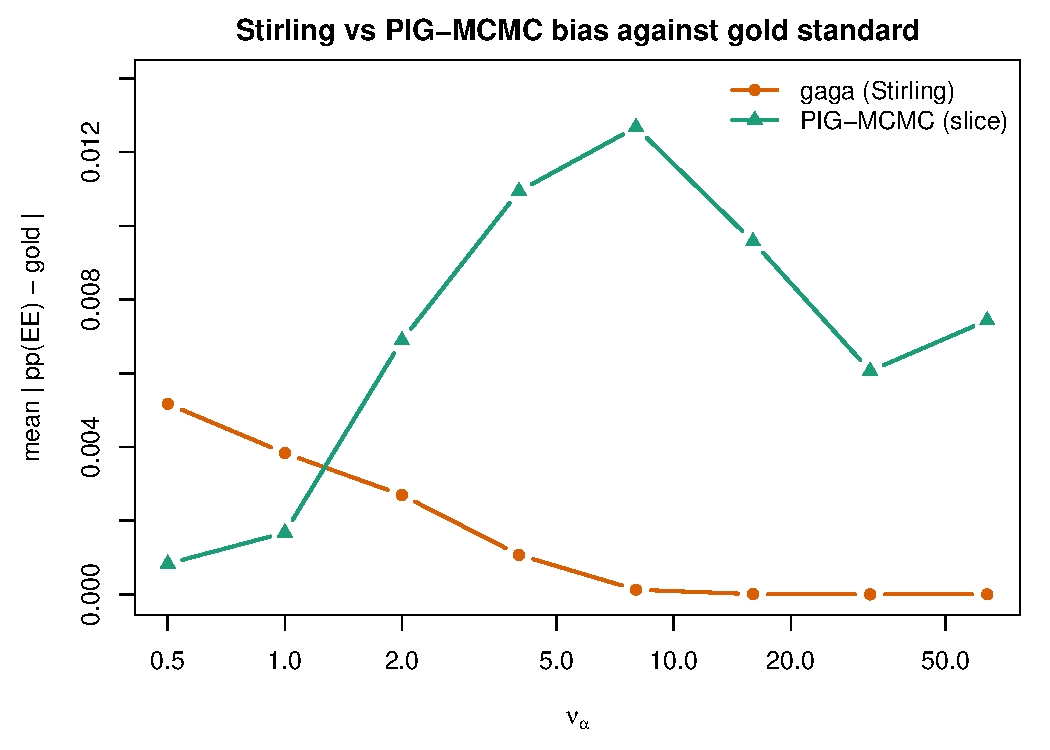
\includegraphics[width=0.78\linewidth]{figs/alpha_sweep_pp_diff.pdf}
\caption{Posterior-probability error against the gold-standard 1D
quadrature, swept over the prior mean $\nu_\alpha$ of the per-gene shape
$\alpha_i$. Same hyperparameters fed to both methods. PIG-MCMC tracks
gold within MCMC noise across the entire range; gaga's Stirling-based
calculation drifts away from gold as $\nu_\alpha \to 0$. The two
strategies cross near $\nu_\alpha \approx 2$.}
\label{fig:gaga.sweep}
\end{figure}

\begin{figure}[t]
\centering
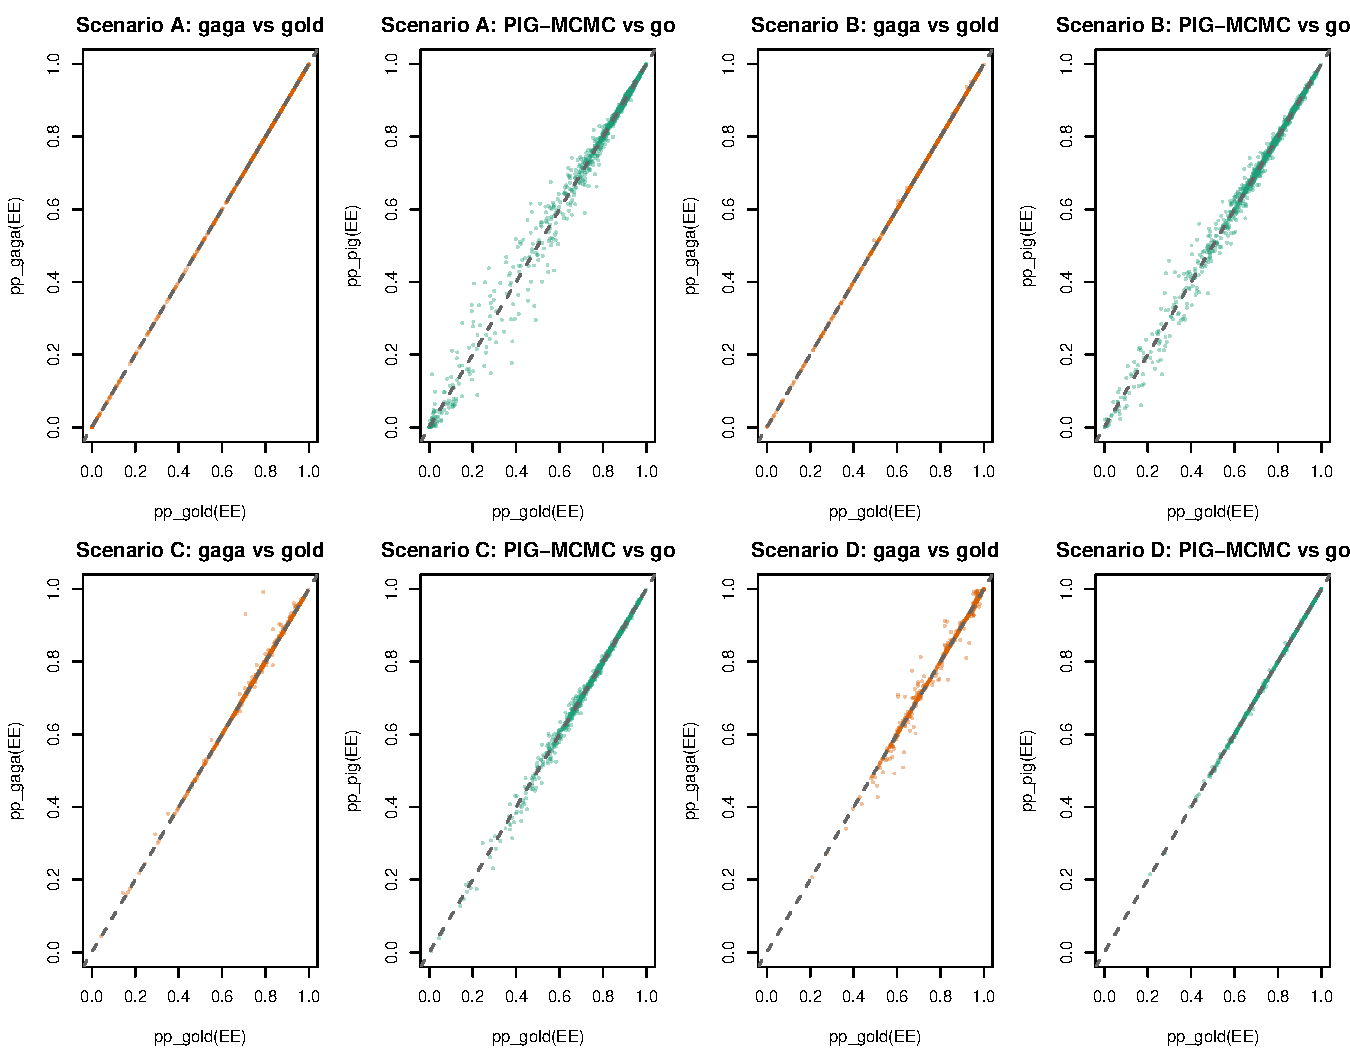
\includegraphics[width=0.95\linewidth]{figs/scatter_pp_vs_gold.pdf}
\caption{Per-gene posterior probabilities of $z_i = 0$ (EE) plotted
against the gold-standard 1D quadrature, for each of the four
simulation scenarios. Left columns: gaga (Stirling); right columns:
PIG-MCMC. Diagonal reference is the perfect-agreement line. In
scenarios A and B, gaga is essentially on the diagonal; in scenarios
C and D, gaga's points fan out, particularly in the small-pp(EE)
region (high-evidence DE genes), while PIG-MCMC remains aligned with
gold up to MCMC noise.}
\label{fig:gaga.scatter}
\end{figure}

\subsubsection{Empirical: Armstrong leukaemia and MAQC}

We follow the two real-data experiments of \citet{Rossell2009GaGa}.
The first is an ALL-versus-MLL classification of acute leukaemia
arrays \citep{Armstrong2002}; the second is the MAQC titration
experiment \citep{MAQC2006} that quotes qPCR measurements for an
external validation set. In both datasets, gaga's
\texttt{quickEM} estimates of $\boldsymbol\theta$ are reused
verbatim, and our PIG-MCMC chain runs for $T=200$ (Schliep mirror)
or $T=150$ (Orange mirror, MAQC) iterations with $T_b = 60$ or $50$
burn-in. We also report \texttt{limma}~\citep{Smyth2004limma} as a
non-Bayesian baseline.

Table~\ref{tab:gaga.empirical} aggregates the comparison. Two
patterns are visible. (i) On the Schliep-mirror Armstrong matrix
(2{,}194 probes), where the data is well-behaved, gaga and
PIG-MCMC call essentially the same DE genes (Jaccard $0.96$,
mean $|\Delta\mathrm{pp}| = 0.011$); the qualitative agreement
matches Table~\ref{tab:gaga.sim.headline}'s scenario A. (ii) On the
Orange-mirror Armstrong matrix (12{,}533 probes) and on MAQC, the
gap is more interesting. The Orange matrix triggers a pathological
quickEM estimate of $\nu_\alpha \approx 8.6\!\times\!10^{10}$,
forcing the per-gene shape posteriors out into the small-effective-$\alpha$
regime where Stirling is least reliable; PIG-MCMC, fed the same
hyperparameter, calls $660$ DE genes against gaga's $388$ ($+70\%$),
and the score correlation drops to $0.95$. On MAQC, the qPCR
validation AUC of PIG-MCMC matches gaga's to four decimal places
($0.9449$), even though the per-probe scores differ by mean
$|\Delta\mathrm{pp}| = 0.20$: this is the regime where the rankings
near the top of the validated-gene list are stable under
Stirling but the absolute posterior probabilities are not.

\begin{table}[t]
\centering
\caption{Empirical comparison of \texttt{gaga::fitGG} (Stirling) and
PIG-MCMC at the same quickEM hyperparameters, on the
\citet{Armstrong2002} leukaemia and \citet{MAQC2006} datasets.
\textit{Schliep} and \textit{Orange} are the two public mirrors of the
Armstrong CEL-derived matrices. The qPCR validation set for MAQC has
1{,}044 assays of which 254 are confirmed differentially expressed
between pools after \texttt{limma}'s F-test at $p < 0.05$.}
\label{tab:gaga.empirical}
\smallskip
\renewcommand{\arraystretch}{1.05}
\setlength{\tabcolsep}{4pt}
{\footnotesize
\begin{tabular}{@{}lccccc@{}}
\toprule
Dataset & metric & gaga & PIG-MCMC & limma & Spearman(PIG, gaga) \\
\midrule
Armstrong (Schliep, $G=2{,}194$) & \#DE @ FDR $0.05$ & 360 & 362 & 361 & $0.997$ \\
Armstrong (Orange, $G=12{,}533$) & \#DE @ FDR $0.05$ & 388 & 660 & 2{,}982 & $0.951$ \\
MAQC ($G=5{,}000$) & qPCR AUC & $0.9449$ & $0.9449$ & $0.9528$ & $0.886$ \\
\bottomrule
\end{tabular}}
\end{table}

The MAQC ROC AUC of $0.9449$ is identical between gaga and PIG-MCMC
to four decimal places, and \texttt{limma} reaches $0.9528$. This
slight \texttt{limma} advantage on MAQC is consistent with what
\citet{Rossell2009GaGa} reported in his Figure~2(b); both Bayesian
methods make their gain on the Armstrong-style benchmark, where the
gene-level shrinkage from $b_\alpha, \nu_\alpha$ matters.

\subsubsection{Discussion}

The simulation gives a clean picture of when the Stirling step in
\citet{Rossell2009GaGa} matters. When $\nu_\alpha \ge 4$ and the
per-cluster sample size $n_c$ is moderate, the gamma approximation to
the GaS density is accurate to machine precision, and our P-IG MCMC
chain at moderate length is uniformly noisier than Stirling at the
same hyperparameters. Conversely, when $\nu_\alpha$ falls below
about $2$, the Stirling error grows past the P-IG MCMC noise floor;
on the extreme single-cell-like scenario D our chain is roughly
five times closer to the gold-standard posterior than Stirling.

The empirical comparison shows that, at the hyperparameters that
\texttt{gaga::fitGG}'s EM produces on real data, the practical
difference is dataset-specific: on the well-behaved Schliep mirror
of Armstrong the two methods are interchangeable, on the
\texttt{just.gcrma}-discordant Orange mirror they diverge sharply,
and on MAQC the validation AUC is identical despite per-probe
posteriors that differ by 20 percentage points. From a software
engineering point of view, the P-IG MCMC option lets a user keep
gaga's hyperparameter EM intact and decide \emph{post hoc} whether
the per-gene posterior step needs the exact treatment.
